% !TeX spellcheck = en_US

\pdfminorversion=4 % for acroread
\ifdefined\ishandout
  \documentclass[aspectratio=169,t,handout,xcolor={usenames,dvipsnames}]{beamer}
\else
  \documentclass[aspectratio=169,t,xcolor={usenames,dvipsnames}]{beamer}
\fi

\usepackage{../beamerstyle}
\usepackage{dsfont}
\usepackage{bm}
\usepackage[english]{babel}
\usepackage[utf8]{inputenc}
\usepackage{graphicx}
\usepackage{algorithm}
\usepackage[ruled,vlined,algo2e,linesnumbered]{algorithm2e}
%\usepackage[boxed,vlined]{algorithm2e}
\usepackage{hyperref}
\usepackage{booktabs}
\usepackage{mathtools}

\usepackage{amsmath,amssymb}
\usepackage{listings}
\lstset{frame=lines,framesep=3pt,numbers=left,numberblanklines=false,basicstyle=\ttfamily\small}

\usepackage{subfig}
\usepackage{multicol}
%\usepackage{appendixnumberbeamer}
%
\usepackage{tcolorbox}

\usepackage{pgfplots}
\usepackage{tikz}
\usetikzlibrary{trees} 
\usetikzlibrary{shapes.geometric}
\usetikzlibrary{positioning,shapes,shadows,arrows,calc,mindmap}
\usetikzlibrary{positioning,fadings,through}
\usetikzlibrary{decorations.pathreplacing}
\usetikzlibrary{intersections}
\usetikzlibrary{positioning,fit,calc,shadows,backgrounds}
\pgfdeclarelayer{background}
\pgfdeclarelayer{foreground}
\pgfsetlayers{background,main,foreground}
\tikzstyle{activity}=[rectangle, draw=black, rounded corners, text centered, text width=8em]
\tikzstyle{data}=[rectangle, draw=black, text centered, text width=8em]
\tikzstyle{myarrow}=[->, thick, draw=black]

% Define the layers to draw the diagram
\pgfdeclarelayer{background}
\pgfdeclarelayer{foreground}
\pgfsetlayers{background,main,foreground}

%\usepackage{listings}
%\lstset{numbers=left,
%  showstringspaces=false,
%  frame={tb},
%  captionpos=b,
%  lineskip=0pt,
%  basicstyle=\ttfamily,
%%  extendedchars=true,
%  stepnumber=1,
%  numberstyle=\small,
%  xleftmargin=1em,
%  breaklines
%}

 
\definecolor{blue}{RGB}{0, 74, 153}

\usetheme{Boadilla}
%\useinnertheme{rectangles}
\usecolortheme{whale}
\setbeamercolor{alerted text}{fg=blue}
\useoutertheme{infolines}
\setbeamertemplate{navigation symbols}{\vspace{-5pt}} % to lower the logo
\setbeamercolor{date in head/foot}{bg=white} % blue
\setbeamercolor{date in head/foot}{fg=blue}
\setbeamercolor{author  in head/foot}{bg=white} %blue
\setbeamercolor{title in head/foot}{bg=white} % blue
\setbeamercolor{title}{fg=white, bg=blue}
\setbeamercolor{block title}{fg=white,bg=blue}
\setbeamercolor{block body}{bg=blue!10}
\setbeamercolor{frametitle}{fg=white, bg=blue}
\setbeamercovered{invisible}

% \makeatletter
% \setbeamertemplate{footline}
% {
%   \leavevmode%
%   \hbox{%
%   \begin{beamercolorbox}[wd=.333333\paperwidth,ht=2.25ex,dp=1ex,center]{author in head/foot}%
% %    \usebeamerfont{author in head/foot}\insertshortauthor
%   \end{beamercolorbox}%
%   \begin{beamercolorbox}[wd=.333333\paperwidth,ht=2.25ex,dp=1ex,center]{title in head/foot}%
%     \usebeamerfont{title in head/foot}\insertshorttitle
%   \end{beamercolorbox}%
%   \begin{beamercolorbox}[wd=.333333\paperwidth,ht=2.25ex,dp=1ex,right]{date in head/foot}%
%     \usebeamerfont{date in head/foot}\insertshortdate{}\hspace*{2em}
% %    \insertframenumber\hspace*{2ex} 
%   \end{beamercolorbox}}%
%   \vskip0pt%
% }
% \makeatother

%\pgfdeclareimage[height=1.2cm]{automl}{images/logos/automl.png}
%\pgfdeclareimage[height=1.2cm]{freiburg}{images/logos/freiburg}

%\logo{\pgfuseimage{freiburg}}

\renewcommand{\comment}[1]{
	\noindent
	%\vspace{0.25cm}
	{\color{red}{\textbf{TODO:} #1}}
	%\vspace{0.25cm}
}
\newcommand{\notefh}[1]{\textcolor{red}{\textbf{FH:} #1}}
\renewcommand{\comment}[1]{}
\newcommand{\hide}[1]{}
\newcommand{\cemph}[2]{\emph{\textcolor{#1}{#2}}}

\newcommand{\lit}[1]{{\footnotesize\color{black!60}[#1]}}

\newcommand{\litw}[1]{{\footnotesize\color{blue!20}[#1]}}


\newcommand{\myframe}[2]{\begin{frame}[c]{#1}#2\end{frame}}
\newcommand{\myframetop}[2]{\begin{frame}{#1}#2\end{frame}}
\newcommand{\myit}[1]{\begin{itemize}#1\end{itemize}}
\newcommand{\myblock}[2]{\begin{block}{#1}#2\end{block}}


\newcommand{\votepurple}[1]{\textcolor{Purple}{$\bigstar$}}
\newcommand{\voteyellow}[1]{\textcolor{Goldenrod}{$\bigstar$}}
\newcommand{\voteblue}[1]{\textcolor{RoyalBlue}{$\bigstar$}}
\newcommand{\votepink}[1]{\textcolor{Pink}{$\bigstar$}}

\newcommand{\diff}{\mathop{}\!\mathrm{d}}
\newcommand{\refstyle}[1]{{\small{\textcolor{gray}{#1}}}}
\newcommand{\hands}[0]{\includegraphics[height=1.5em]{images/hands}}
\newcommand{\transpose}[0]{{\textrm{\tiny{\sf{T}}}}}
\newcommand{\norm}{{\mathcal{N}}}
\newcommand{\cutoff}[0]{\kappa}
\newcommand{\instD}[0]{\dataset}
\newcommand{\insts}[0]{\mathcal{I}}
\newcommand{\inst}[0]{i}
\newcommand{\instI}[1]{i^{(#1)}}

% Iteration specific instance of variable/function/anything
% Introduced in the BO section, but moved up here to make it available within other macros
\newcommand{\iter}[2][\bocount]{{#2}^{(#1)}}

%--------HPO parameter macros-----------

% Parameter Configuration Space
\newcommand{\pcs}[0]{\pmb{\Lambda}}

% ???
\newcommand{\bx}[0]{\conf}

% Parameter Configuration
\newcommand{\conf}[0]{\pmb{\lambda}}

% Final Configuration
\newcommand{\finconf}[0]{\pmb{\hat{\lambda}}}

% Configuration corresponding to a given iteration -- better use \iter!
\newcommand{\confI}[1]{{\conf}^{(#1)}}

% Default Configuration
\newcommand{\defconf}[0]{{\conf}_{\text{def}}}

% Incumbent Configuration
\newcommand{\incumbent}[1][\bocount]{\iter[#1]{\finconf}}

% Optimal Configuration
\newcommand{\optconf}[0]{{\conf}^*}

% Configuration Space
\newcommand{\confs}[0]{\pcs}

%----------------------------------------

%\newcommand{\vlambda}[0]{\bm{\lambda}}
%\newcommand{\vLambda}[0]{\bm{\Lambda}}
\newcommand{\dataset}[0]{\mathcal{D}}
\newcommand{\datasets}[0]{\mathbf{D}}
\newcommand{\loss}[0]{L}
\newcommand{\risk}{\mathcal{R}}
\newcommand{\riske}{\mathcal{R}_{\text{emp}}}
\newcommand{\cost}[0]{c}
\newcommand{\costI}[1]{c^{(#1)}}

% Gaussian Process
\newcommand{\gp}{\mathcal{G}}
% Family of Objective Functions
\newcommand{\objF}{F}

%---------------BO Macros------------------

% BO loop counter
\newcommand{\bocount}{t}
% BO loop counter max, the counter runs from 1 to this value
\newcommand{\bobudget}{T}
% BO loop observation
\newcommand{\obs}[1][\conf]{\cost({#1})}
% BO loop observation space
\newcommand{\obsspace}{\mathcal{Y}}
% BO loop next observation
\newcommand{\bonextobs}{\obs[\iter{\conf}]}
% Acquisition Function, no args
\newcommand{\acq}{u}
% Standard Normal PDF
\newcommand{\pdf}{\phi}
% Standard Normal CDF
\newcommand{\cdf}{\Phi}
% Mean
\newcommand{\mean}{\mu}
% Standard Deviation
\newcommand{\stddev}{\sigma}
% Variance
\newcommand{\variance}{\sigma^2}
% Noise
\newcommand{\noise}{\nu}
% BO loop next selected sample
\newcommand{\bonextsample}{\confI{\bocount}}

% Single hyperparameter
\newcommand{\hyperparam}{\lambda}

% Single hyperparameter within a hyperparameter configuration
\newcommand{\hyperparami}[1][i]{{\hyperparam}_#1}

% Full definition of final configuration
\newcommand{\finconffull}{\incumbent[\bobudget]}

% Dataset
\newcommand{\datasetHPO}{{\dataset}_{HPO}}

% Dataset definition
\newcommand{\datasetHPOdef}{{\langle \bonextsample,\,\bonextobs \rangle}_{\bocount=1}^{\bobudget}}

% Double Display Fraction, forces large displays for everything in numerator and denominator
\newcommand\ddfrac[2]{\frac{\displaystyle #1}{\displaystyle #2}}

% Conditional Probability "Given That" Relation, source:https://tex.stackexchange.com/a/141685/205886
\newcommand\given[1][]{\:#1\vert\:}

% Expectation as a math operator
\DeclareMathOperator*{\E}{\mathbb{E}}

% Citation 
\newcommand{\source}[1]{
    \begin{flushright}
    	Source: \lit{#1}
    \end{flushright}
}
%-------------------------------------------

%Real numbers set
\newcommand{\realnum}{\mathbb{R}}
%Configuration space - do not use
%\newcommand{\configspace}{\Theta}
%Instances - do not use
%\newcommand{\instances}{\mathcal{I}}
%Expected value
\newcommand{\expectation}{\mathbb{E}}
%Kernel
\newcommand{\kernel}{\kappa}
%Constraint function
\newcommand{\constraintf}{c}
%Normal distribution
\newcommand{\normaldist}{\mathcal{N}}

% \renewcommand{\vec}[1]{\mathbf{#1}}
\newcommand{\hist}[0]{\dataset_{\text{Hist}}}
\newcommand{\param}[0]{p}
\newcommand{\algo}[0]{\mathcal{A}}
\newcommand{\algos}[0]{\mathbf{A}}
%\newcommand{\nn}[0]{N}
\newcommand{\feats}[0]{\mathcal{X}_{\text{meta}}}
\newcommand{\feat}[0]{\x_{\text{meta}}}
%\newcommand{\cluster}[0]{\vec{h}}
%\newcommand{\clusters}[0]{\vec{H}}
\newcommand{\perf}[0]{\mathbb{R}}
%\newcommand{\surro}[0]{\mathcal{S}}
\newcommand{\surro}[0]{\hat{\cost}}
\newcommand{\func}[0]{f}
\newcommand{\epm}[0]{\surro}
\newcommand{\portfolio}[0]{\mathbf{P}}
\newcommand{\schedule}[0]{\mathcal{S}}

% Machine Learning
\newcommand{\mdata}[0]{\dataset_{\text{meta}}}
\newcommand{\datasettrain}[0]{\dataset_{\text{train}}}
\newcommand{\datasetval}[0]{\dataset_{\text{val}}}
\newcommand{\datasettest}[0]{\dataset_{\text{test}}}
\newcommand{\x}[0]{\mathbf{x}}
\newcommand{\y}[0]{y}
\newcommand{\xI}[1]{\mathbf{x}^{(#1)}}
\newcommand{\yI}[1]{y^{(#1)}}
\newcommand{\fx}{f(\mathbf{x})}  % f(x), continuous prediction function
\newcommand{\Hspace}{\mathcal{H}} % hypothesis space where f is from
\newcommand{\fh}{\hat{f}}       % f hat, estimated prediction function

% Deep Learning
\newcommand{\weights}[0]{\theta}
\newcommand{\metaweights}[0]{\phi}


% reinforcement learning
\newcommand{\policies}[0]{\mathbf{\Pi}}
\newcommand{\policy}[0]{\pi}
\newcommand{\actionRL}[0]{a}
\newcommand{\stateRL}[0]{s}
\newcommand{\statesRL}[0]{\mathcal{S}}
\newcommand{\rewardRL}[0]{r}
\newcommand{\rewardfuncRL}[0]{\mathcal{R}}

\RestyleAlgo{algoruled}
\DontPrintSemicolon
\LinesNumbered
\SetAlgoVlined
\SetFuncSty{textsc}

\SetKwInOut{Input}{Input}
\SetKwInOut{Output}{Output}
\SetKw{Return}{return}

%\newcommand{\changed}[1]{{\color{red}#1}}

%\newcommand{\citeN}[1]{\citeauthor{#1}~(\citeyear{#1})}

\renewcommand{\vec}[1]{\mathbf{#1}}
\DeclareMathOperator*{\argmin}{arg\,min}
\DeclareMathOperator*{\argmax}{arg\,max}

%\newcommand{\aqme}{\textit{AQME}}
%\newcommand{\aslib}{\textit{ASlib}}
%\newcommand{\llama}{\textit{LLAMA}}
%\newcommand{\satzilla}{\textit{SATzilla}}
%\newcommand{\satzillaY}[1]{\textit{SATzilla'{#1}}}
%\newcommand{\snnap}{\textit{SNNAP}}
%\newcommand{\claspfolioTwo}{\textit{claspfolio~2}}
%\newcommand{\flexfolio}{\textit{FlexFolio}}
%\newcommand{\claspfolioOne}{\textit{claspfolio~1}}
%\newcommand{\isac}{\textit{ISAC}}
%\newcommand{\eisac}{\textit{EISAC}}
%\newcommand{\sss}{\textit{3S}}
%\newcommand{\sunny}{\textit{Sunny}}
%\newcommand{\ssspar}{\textit{3Spar}}
%\newcommand{\cshc}{\textit{CSHC}}
%\newcommand{\cshcpar}{\textit{CSHCpar}}
%\newcommand{\measp}{\textit{ME-ASP}}
%\newcommand{\aspeed}{\textit{aspeed}}
%\newcommand{\autofolio}{\textit{AutoFolio}}
%\newcommand{\cedalion}{\textit{Cedalion}}
\newcommand{\fanova}{\textit{fANOVA}}
\newcommand{\sbs}{\textit{SB}}
\newcommand{\oracle}{\textit{VBS}}

% like approaches
\newcommand{\claspfoliolike}[1]{\texttt{claspfolio-#1-like}}
\newcommand{\satzillalike}[1]{\texttt{SATzilla'#1-like}}
\newcommand{\isaclike}{\texttt{ISAC-like}}
\newcommand{\ssslike}{\texttt{3S-like}}
\newcommand{\measplike}{\texttt{ME-ASP-like}}

\newcommand{\irace}{\textit{I/F-race}}
\newcommand{\gga}{\textit{GGA}}
\newcommand{\smac}{\textit{SMAC}}
\newcommand{\paramils}{\textit{ParamILS}}
\newcommand{\spearmint}{\textit{Spearmint}}
\newcommand{\tpe}{\textit{TPE}}


\usepackage{pifont}
\newcommand{\itarrow}{\mbox{\Pisymbol{pzd}{229}}}
\newcommand{\ithook}{\mbox{\Pisymbol{pzd}{52}}}
\newcommand{\itcross}{\mbox{\Pisymbol{pzd}{56}}}
\newcommand{\ithand}{\mbox{\raisebox{-1pt}{\Pisymbol{pzd}{43}}}}

%\DeclareMathOperator*{\argmax}{arg\,max}

\newcommand{\ie}{{\it{}i.e.\/}}
\newcommand{\eg}{{\it{}e.g.\/}}
\newcommand{\cf}{{\it{}cf.\/}}
\newcommand{\wrt}{\mbox{w.r.t.}}
\newcommand{\vs}{{\it{}vs\/}}
\newcommand{\vsp}{{\it{}vs\/}}
\newcommand{\etc}{{\copyedit{etc.}}}
\newcommand{\etal}{{\it{}et al.\/}}

\newcommand{\pscProc}{{\bf procedure}}
\newcommand{\pscBegin}{{\bf begin}}
\newcommand{\pscEnd}{{\bf end}}
\newcommand{\pscEndIf}{{\bf endif}}
\newcommand{\pscFor}{{\bf for}}
\newcommand{\pscEach}{{\bf each}}
\newcommand{\pscThen}{{\bf then}}
\newcommand{\pscElse}{{\bf else}}
\newcommand{\pscWhile}{{\bf while}}
\newcommand{\pscIf}{{\bf if}}
\newcommand{\pscRepeat}{{\bf repeat}}
\newcommand{\pscUntil}{{\bf until}}
\newcommand{\pscWithProb}{{\bf with probability}}
\newcommand{\pscOtherwise}{{\bf otherwise}}
\newcommand{\pscDo}{{\bf do}}
\newcommand{\pscTo}{{\bf to}}
\newcommand{\pscOr}{{\bf or}}
\newcommand{\pscAnd}{{\bf and}}
\newcommand{\pscNot}{{\bf not}}
\newcommand{\pscFalse}{{\bf false}}
\newcommand{\pscEachElOf}{{\bf each element of}}
\newcommand{\pscReturn}{{\bf return}}

%\newcommand{\param}[1]{{\sl{}#1}}
\newcommand{\var}[1]{{\it{}#1}}
\newcommand{\cond}[1]{{\sf{}#1}}
%\newcommand{\state}[1]{{\sf{}#1}}
%\newcommand{\func}[1]{{\sl{}#1}}
\newcommand{\set}[1]{{\Bbb #1}}
%\newcommand{\inst}[1]{{\tt{}#1}}
\newcommand{\myurl}[1]{{\small\sf #1}}

\newcommand{\Nats}{{\Bbb N}}
\newcommand{\Reals}{{\Bbb R}}
\newcommand{\extset}[2]{\{#1 \; | \; #2\}}

\newcommand{\vbar}{$\,\;|$\hspace*{-1em}\raisebox{-0.3mm}{$\,\;\;|$}}
\newcommand{\vendbar}{\raisebox{+0.4mm}{$\,\;|$}}
\newcommand{\vend}{$\,\:\lfloor$}


\newcommand{\goleft}[2][.7]{\parbox[t]{#1\linewidth}{\strut\raggedright #2\strut}}
\newcommand{\rightimage}[2][.3]{\mbox{}\hfill\raisebox{1em-\height}[0pt][0pt]{\includegraphics[width=#1\linewidth]{#2}}\vspace*{-\baselineskip}}





\title[AutoML: Capping]{AutoML: Beyond AutoML}
\subtitle{Per-Instance Algorithm Configuration}
\author[Marius Lindauer]{Bernd Bischl \and Frank Hutter \and Lars Kotthoff\newline \and \underline{Marius Lindauer} \and Joaquin Vanschoren}
\institute{}
\date{}



% \AtBeginSection[] % Do nothing for \section*
% {
%   \begin{frame}{Outline}
%     \bigskip
%     \vfill
%     \tableofcontents[currentsection]
%   \end{frame}
% }

\begin{document}
	
	\maketitle
	

%----------------------------------------------------------------------
\begin{frame}[c]{Homogeneous vs. Heterogeneous Instances}

\begin{block}{Assumption of AC: Homogeneous Instance Distribution}
	\begin{itemize}
		\item Algorithm configuration tools assume that the \alert{instance distribution is homogeneous}\\ (see video on "Best Practices for AC")
		\smallskip
		\item Important because
		\begin{itemize}
			\item there is a well-performing configuration for all (or most) instances
			\item the racing algorithm can make educated decisions on subsets
		\end{itemize}
	\end{itemize}
\end{block}

\medskip
\pause

\begin{block}{Violated assumption of AC: Hetergeneous Instance Distribution}
	\begin{itemize}
		\item The racing algorithm will make inconsistent (or even wrong) decisions 
		\item There is no single well-performing configuration for all instances
	\end{itemize}
\end{block}

\pause
\medskip
$\leadsto$ What should we do with heterogeneous instance distributions?

\end{frame}
%-----------------------------------------------------------------------

%----------------------------------------------------------------------
\begin{frame}[c]{Why are systems for heterogeneous instance distributions important?}

\begin{enumerate}
	\item We cannot guarantee homogeneity in practice
	\begin{enumerate}
		\item Instances might get larger and harder
		\item The underlying task or business case might change
	\end{enumerate}
	\medskip
	\pause
	\item We don't want to do algorithm configuration always from scratch
	\medskip
	\pause
	\item An adaptive configuration system would be the holy grail 
	\begin{itemize}
		\item[$\leadsto$] hard to achieve
 	\end{itemize}
\end{enumerate}


\end{frame}
%-----------------------------------------------------------------------
%----------------------------------------------------------------------
\begin{frame}[c]{PIAC: Per-Instance Algorithm Configuration}

\centering
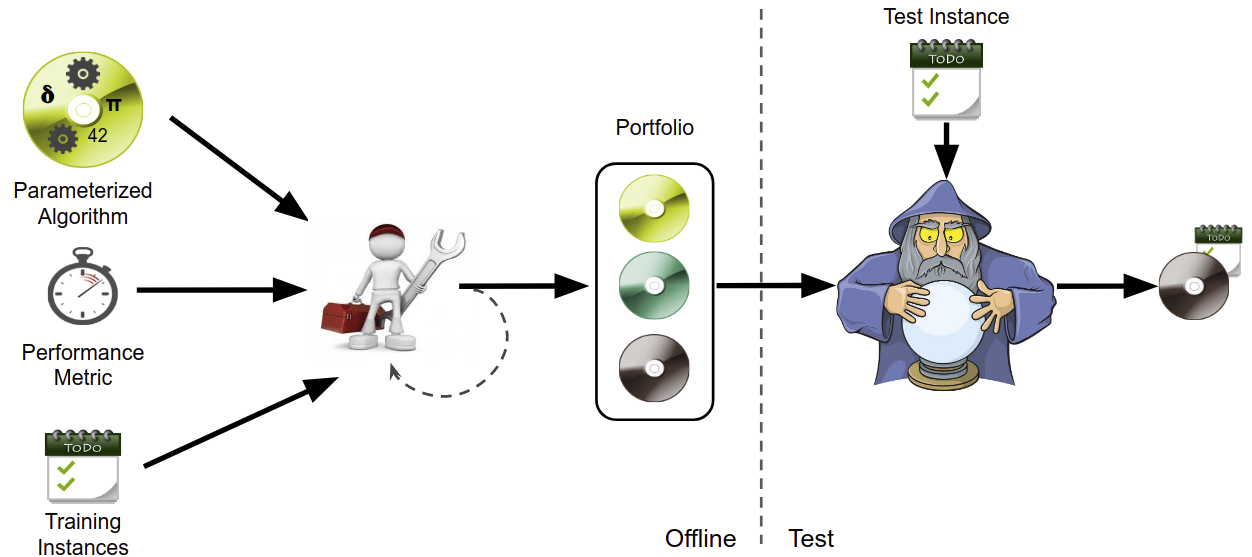
\includegraphics[width=0.75\textwidth]{images/piac_full_comic}

\pause
\bigskip

\begin{itemize}
	\item You can use whichever kind of algorithm selection (wizard) you want
	\item \alert{Challenge:} Building a portfolio
	\item \alert{Use case:} Instances are heterogeneous
\end{itemize}

\end{frame}
%----------------------------------------------------------------------
%----------------------------------------------------------------------
\begin{frame}[c]{PIAC: Manual Expert Approach}

\begin{block}{Basic Assumption}
Heterogeneous instance set can be divided into homogeneous subsets
\end{block}

\pause
\bigskip

\begin{block}{Manual Expert}
\begin{itemize}
\item An expert knows the homogeneous subsets (e.g., origin of instances)
\item Determine a well-performing configuration on each subset\\
$\to$ portfolio of configurations
\item Use Algorithm Selection to select a well-performing configuration on each instance 
\end{itemize}

\end{block}  

\end{frame}
%----------------------------------------------------------------------
%----------------------------------------------------------------------
\begin{frame}{Instance-Specific Algorithm Configuration: ISAC{} \litw{\href{https://wiwi.uni-paderborn.de/fileadmin/dep3ls7/Downloads/Publikationen/PDFs/isac-ecai2010.pdf}{Kadioglu et al. 2010}}}


\begin{block}{Idea}
Training:
\begin{enumerate}
\item Cluster instances into homogeneous subsets\\ (using $g$-means in the instance feature space)
\item Apply algorithm configuration (here GGA) on each instance set
\end{enumerate}

\pause
Test:
\begin{enumerate}
\item Determine the nearest cluster ($k$-NN with $k=1$) in feature space
\item Apply optimized configuration of this cluster 
\end{enumerate}
\end{block}

\begin{center}
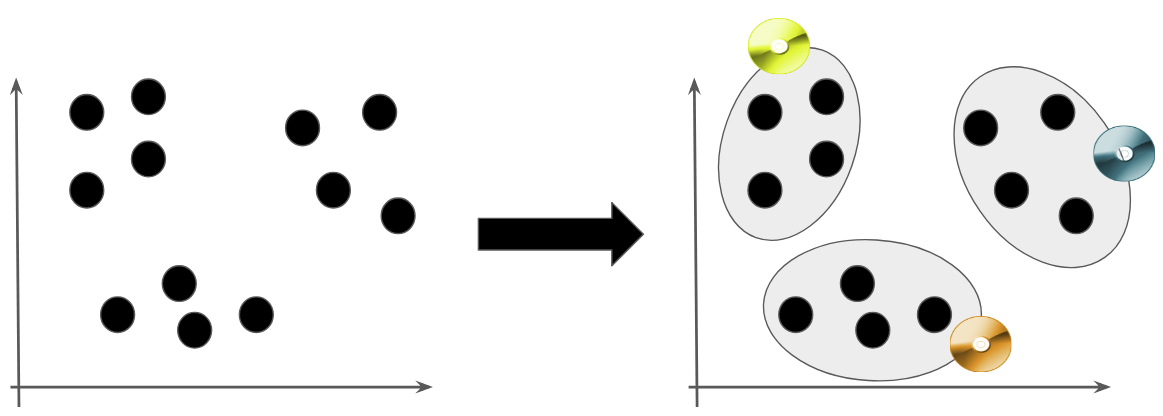
\includegraphics[width=.3\textwidth]{images/isac}
\end{center}

\end{frame}
%----------------------------------------------------------------------
%----------------------------------------------------------------------
%\begin{frame}[c]{EISAC{}~\litw{Y. Malitsky et al. 2013}}
%
%\begin{block}{Motivation}
%\begin{itemize}
%\item Over time, the underlying distribution of $\insts$ changes
%\item All-encompassing training set does not exist
%\item Selector should evolve over time
%\end{itemize}
%\end{block}
%
%\bigskip
%\pause
%
%\begin{block}{Idea}
%\begin{itemize}
%\item Update cluster if we see instances that are not represented 
%\item Update configuration selection for a cluster if a cluster gets more instances
%\item Add and remove configurations, and update clusters
%\end{itemize}
%\end{block}
%
%\end{frame}
%----------------------------------------------------------------------
%----------------------------------------------------------------------
%\begin{frame}[c]{ISAC{}+ \litw{Y. Malitsky et al. 2014}}
%
%\begin{block}{Observations}
%\begin{itemize}
%\item Not important to apply the configuration found on a cluster
%\item Arbitrary algorithm selection approach possible 
%\end{itemize}
%\end{block}
%
%\pause
%\medskip
%
%\begin{block}{Idea}
%\begin{enumerate}
%\item Cluster instances
%\item Apply algorithm configuration on each cluster
%\item Assess the performance of all configurations on each instance
%\item Use cost-sensitive hierarchical clustering (CSHC; see lecture on AS)
%\end{enumerate}
%\end{block}
%
%\end{frame}
%----------------------------------------------------------------------
%----------------------------------------------------------------------
\begin{frame}[c]{Hydra~\litw{\href{https://www.aaai.org/ocs/index.php/AAAI/AAAI10/paper/view/1929/1960}{Xu et al. 2010}}}

\begin{block}{Idea}
\begin{itemize}
\item Iteratively add configurations to a portfolio $\portfolio$, start with $\portfolio = \emptyset$
\item In each iteration, determine configuration that is complementary to~$\portfolio$
\begin{itemize}
\item[$\leadsto$] Maximize marginal contribution to $\portfolio$
\end{itemize}
\end{itemize}

\pause

Marginal contribution of a configuration $\conf$ to a portfolio $\portfolio$:
\begin{equation}
c(\portfolio) -  c(\portfolio \cup \{\conf\})  \nonumber
\end{equation}

\end{block}

\pause

\scalebox{0.7}{
%\begin{center}
	\begin{tikzpicture}[node distance=5cm, thick]
	%PreProcessing
	%\node (Algo) [data] {Algorithm $A$};
	\node (Data) [data] {Instances $\insts$};
	\node (CS) [data, right of=Data, xshift=-0.5cm] {Algorithm $\algo$ and\\ its Configuration\\ Space $\confs$};
	\node (Select) [activity, below of=Data, node distance=2.0cm] {Select $\conf \in \confs$\\ and $\inst \in \insts$};
	\node (Run) [activity, right of=Select, xshift=-0.5cm] {\only<2-3>{Assess\\ $\algo(\conf)$ on $\inst$}%
															\only<4-5>{Assess $\algo(\conf||\conf_1)$ on $\inst$}
															\only<6-6>{Assess $\algo(\conf||\conf_1||\conf_2)$ on $\inst$}};
	%\node (Return) [activity, right of=Run, text width=9em] {Return Performance\\ of $A(c)$ on $I'$}; 
	%\node (Data) [data, left of=Select] {Instances $I$};	
	\node (Result) [data, right of=Run, node distance=5.5cm] { $\portfolio = $\only<2-2>{$\{\}$}%
																\only<3-4>{$\{\conf_1\}$}%
																\only<5->{$\{\conf_1,\conf_2\}$}%
																}; 
	
	\draw[myarrow] (Data) -- ($(Select)+(-0.0,+0.8)$);
	\draw[myarrow] (CS) -- ($(Run)+(-0.0,+0.8)$);
	%\draw[myarrow] (Data) -- ($(Select)+(-2.1,+0.0)$);
	
	%\draw[thick, dashed] (Algo) -- (CS);
	\only<3-3>{\draw[myarrow] ($(Run.east)+(0.25,.1)$) to [bend angle=60, bend left] node[above] {\footnotesize $\conf_1$} ($(Result.west)+(0.0,.1)$);}
	\only<5-5>{\draw[myarrow] ($(Run.east)+(0.25,.1)$) to [bend angle=60, bend left] node[above] {\footnotesize $\conf_2$} ($(Result.west)+(0.0,.1)$);}
	\only<2-2>{\draw[myarrow] ($(Result.west)+(0.0,-.1)$) to [bend angle=60, bend left] node[below] {\footnotesize $\{\}$} ($(Run.east)+(0.25,-.1)$);}
	\only<4-4>{\draw[myarrow] ($(Result.west)+(0.0,-.1)$) to [bend angle=60, bend left] node[below] {\footnotesize $\{\conf_1\}$} ($(Run.east)+(0.25,-.1)$);}
	\only<6-6>{\draw[myarrow] ($(Result.west)+(0.0,-.1)$) to [bend angle=60, bend left] node[below] {\footnotesize $\{\conf_1,\conf_2\}$} ($(Run.east)+(0.25,-.1)$);}
	\draw[myarrow] (Select) -- (Run);
	%\draw[myarrow] (Run) -- (Return);
	\draw[myarrow] (Run.south) |- ++(0.0,-0.8)  node[above, xshift=-2.2cm] {Return $\min\left\{c(\theta), c(\portfolio) \right\}$} -| (Select.south);
	
	\begin{pgfonlayer}{background}
    
        % Configuration Process
    	\path (Select -| Select.west)+(-0.25,0.85) node (resUL) {};
    	\path (Run.east |- Run.south)+(0.25,-1.3) node(resBR) {};
    	\path [rounded corners, draw=black!20, dashed] (resUL) rectangle (resBR);
		\path (Run.east |- Run.south)+(-1.5,-1.1) node [text=black!60] {Configuration Task};
    	
    \end{pgfonlayer}
	
\end{tikzpicture}
	
%\end{center}

}

\end{frame}
%----------------------------------------------------------------------
%----------------------------------------------------------------------
% !TeX spellcheck = en_US
\begin{frame}[c]{Heterogeneous example}
	\begin{figure}
		\centering
			\begin{tikzpicture}
			%	\draw[very thin,color=gray] (-0.1,-1.1) grid (3.9,3.9);
			\draw[->] (-0.2,0) -- (4.2,0) node[right] {${\conf}$};
			\draw[->] (0,-0.2) -- (0,4.2) node[above] {$c_{\inst_i}({\conf})$};
			\draw[color=blue,domain=3:7]   plot (\x-3,{sin((\x-2) r) + 1.275})   node[right] {$\inst_0({\conf})$};
			\draw[color=orange,domain=0:4] plot (\x,{0.05*exp(\x)}) node[right] {$\inst_1({\conf})$};
			\draw[color=red,domain=-2:2] plot (\x+2,{\x*\x}) node[right] {$\inst_2({\conf})$};
			
			\only<2->{
				 \foreach \x/\xtext in {0/{\conf}_{\inst_1}^*, 2/{\conf}_{\inst_2}^*, 3.725/{\conf}_{\inst_0}^*}
					\draw[shift={(\x,0)}] (0pt,2pt) -- (0pt,-2pt) node[below] {$\xtext$};
			}
			\only<3->{
				 \foreach \y/\ytext in {.75/c_{{\conf}_{SB}}}
					\draw[shift={(0,\y)}] (2pt,0pt) -- (-2pt,0pt) node[left] {$\ytext$};
				 \foreach \x/\xtext in {2.725/{\conf}_{SB}}
					\draw[shift={(\x,0)}] (0pt,2pt) -- (0pt,-2pt) node[below] {$\xtext$};
				 \draw[densely dotted,color=gray] (0,0.75) -- (2.725,.75);
				 \draw[densely dotted,color=gray] (2.725,0) -- (2.725,.75);
			}
			\only<4->{
			%	\draw[dashed,color=gray] (0,0.1275) -- (3.725,0.1275);
				\foreach \y/\ytext in {0.1275/c_{oracle}}
				\draw[shift={(0,\y)}] (2pt,0pt) -- (-2pt,0pt) node[left] {$\ytext$};
			}
			\end{tikzpicture}
	\end{figure}
\end{frame}

\begin{frame}[c]{Hydra: Iteration 1}
		\centering
		\begin{tikzpicture}
		
			\only<1>{
				%	\draw[very thin,color=gray] (-0.1,-1.1) grid (3.9,3.9);
				\draw[->] (-0.2,0) -- (4.2,0) node[right] {${\conf}$};
				\draw[->] (0,-0.2) -- (0,4.2) node[above] {$c_{\inst_i}({\conf})$};
				\draw[color=blue,domain=3:7]   plot (\x-3,{sin((\x-2) r) + 1.275})   node[right] {$\inst_0({\conf})$};
				\draw[color=orange,domain=0:4] plot (\x,{0.05*exp(\x)}) node[right] {$\inst_1({\conf})$};
				\draw[color=red,domain=-2:2] plot (\x+2,{\x*\x}) node[right] {$\inst_2({\conf})$};
				
%				\foreach \y/\ytext in {.75/c_{{\conf}_{0}}}
%				\draw[shift={(0,\y)}] (2pt,0pt) -- (-2pt,0pt) node[left] {$\ytext$};
				\foreach \x/\xtext in {2.725/{\conf}_{0}}
				\draw[shift={(\x,0)}] (0pt,2pt) -- (0pt,-2pt) node[below] {$\xtext$};
%				\draw[densely dotted,color=gray] (0,0.75) -- (2.725,.75);
				\draw[densely dotted,color=gray] (2.725,0) -- (2.725,4);
			}
			\only<2>{
				%Update metric
				%	\draw[very thin,color=gray] (-0.1,-1.1) grid (3.9,3.9);
				\draw[->] (-0.2,0) -- (4.2,0) node[right] {${\conf}$};
				\draw[->] (0,-0.2) -- (0,4.2) node[above] {$c_{\inst_i}^{'}({\conf})$};
				
				\draw[color=orange,domain=0:2.725] plot (\x,{0.05*exp(\x)});
				\draw[color=orange,domain=2.725:4] plot (\x,.75) node[right] {$\inst_1({\conf})$};
				
				\draw[color=red,domain=-.725:.725] plot (\x+2,{\x*\x});
				\draw[color=red,domain=-2:-.725] plot (\x+2,0.525625);
				\draw[color=red,domain=.725:2] plot (\x+2,0.525625) node[right] {$\inst_2({\conf})$};
				
				\draw[color=blue,domain=5.725:7]   plot (\x-3,{sin((\x-2) r) + 1.275})   node[right] {$\inst_0({\conf})$};
				\draw[color=blue,domain=3:5.725]   plot (\x-3,.75);
				
				\foreach \y/\ytext in {.75/c^{'}_{\inst_{\left\{0, 1\right\}}}(\portfolio)}
				\draw[shift={(0,\y)}] (2pt,0pt) -- (-2pt,0pt) node[left,yshift=0.15cm] {$\ytext$};
				\foreach \y/\ytext in {0.525625/c^{'}_{\inst_{2}}(\portfolio)}
				\draw[shift={(0,\y)}] (2pt,0pt) -- (-2pt,0pt) node[left,yshift=-0.15cm] {$\ytext$};
				
				\foreach \x/\xtext in {2.725/{\conf}_{0}}
				\draw[shift={(\x,0)}] (0pt,2pt) -- (0pt,-2pt) node[below] {$\xtext$};
				
%				\draw[densely dotted,color=gray] (0,0.75) -- (2.725,.75);
				\draw[densely dotted,color=gray] (2.725,0) -- (2.725,.75);
			}
		\end{tikzpicture}

			\only<1>{Search initial well performing configuration. Add ${\conf}_{0}$ to $\portfolio$}
			\only<2>{Update metric}
\end{frame}



\begin{frame}[c]{Hydra: Iteration 2}
	\centering
	\begin{tikzpicture}
	\only<1>{
		%Update metric
		%	\draw[very thin,color=gray] (-0.1,-1.1) grid (3.9,3.9);
		\draw[->] (-0.2,0) -- (4.2,0) node[right] {${\conf}$};
		\draw[->] (0,-0.2) -- (0,4.2) node[above] {$c_{\inst_i}^{'}({\conf})$};
		
		\draw[color=orange,domain=0:2.725] plot (\x,{0.05*exp(\x)});
		\draw[color=orange,domain=2.725:4] plot (\x,.75) node[right] {$\inst_1({\conf})$};
		
		\draw[color=red,domain=-.725:.725] plot (\x+2,{\x*\x});
		\draw[color=red,domain=-2:-.725] plot (\x+2,0.525625);
		\draw[color=red,domain=.725:2] plot (\x+2,0.525625) node[right] {$\inst_2({\conf})$};
		
		\draw[color=blue,domain=5.725:7]   plot (\x-3,{sin((\x-2) r) + 1.275})   node[right] {$\inst_0({\conf})$};
		\draw[color=blue,domain=3:5.725]   plot (\x-3,.75);
		
		\foreach \y/\ytext in {.75/}
		\draw[shift={(0,\y)}] (2pt,0pt) -- (-2pt,0pt) node[left,yshift=0.15cm] {$\ytext$};
		\foreach \y/\ytext in {0.525625/}
		\draw[shift={(0,\y)}] (2pt,0pt) -- (-2pt,0pt) node[left,yshift=-0.15cm] {$\ytext$};
		
		\foreach \x/\xtext in {2.725/{\conf}_{0}, 3.725/{\conf}_{1}}
		\draw[shift={(\x,0)}] (0pt,2pt) -- (0pt,-2pt) node[below] {$\xtext$};
		
%		\draw[densely dotted,color=gray] (0,0.75) -- (2.725,.75);
		\draw[densely dotted,color=gray] (2.725,0) -- (2.725,.75);
		\draw[densely dotted,color=gray] (3.725,0) -- (3.725,4);
	}

	\only<2>{
		%Update metric
		%	\draw[very thin,color=gray] (-0.,-.) grid (3.9,3.9);
		\draw[->] (-0.2,0) -- (4.2,0) node[right] {${\conf}$};
		\draw[->] (0,-0.2) -- (0,4.2) node[above] {$c_{\inst_i}^{''}({\conf})$};
		
		\draw[color=orange,domain=0:2.725] plot (\x,{0.05*exp(\x)});
		\draw[color=orange,domain=2.725:4] plot (\x,.75) node[right] {$\inst_({\conf})$};
		
		\draw[color=red,domain=-.725:.725] plot (\x+2,{\x*\x});
		\draw[color=red,domain=-2:-.725] plot (\x+2,0.525625);
		\draw[color=red,domain=.725:2] plot (\x+2,0.525625) node[right] {$\inst_2({\conf})$};
		
		\draw[color=blue,domain=0:4]   plot (\x,.25)   node[right] {$\inst_0({\conf})$};
%		\draw[color=blue,domain=3:5.725]   plot (\x-3,.75);
		
		\foreach \y/\ytext in {.75/}
		\draw[shift={(0,\y)}] (2pt,0pt) -- (-2pt,0pt) node[left,yshift=0.cm] {$\ytext$};
		\foreach \y/\ytext in {0.525625/}
		\draw[shift={(0,\y)}] (2pt,0pt) -- (-2pt,0pt) node[left,yshift=-0.0cm] {$\ytext$};
		\foreach \y/\ytext in {0.25/}
		\draw[shift={(0,\y)}] (2pt,0pt) -- (-2pt,0pt) node[left,yshift=-0.0cm] {$\ytext$};
		
		\foreach \x/\xtext in {2.725/{\conf}_{0}, 3.725/{\conf}_{1}}
		\draw[shift={(\x,0)}] (0pt,2pt) -- (0pt,-2pt) node[below] {$\xtext$};
		
				\draw[densely dotted,color=gray] (0,0.75) -- (2.725,.75);
		\draw[densely dotted,color=gray] (2.725,0) -- (2.725,.75);
		\draw[densely dotted,color=gray] (3.725,0) -- (3.725,.25);
	}
	\end{tikzpicture}
	
		\only<1>{Search well performing configuration complementary to $\portfolio$.\\Add ${\conf}_{1}$ to $\portfolio$.}
		\only<2>{Update metric}
\end{frame}
%----------------------------------------------------------------------
%----------------------------------------------------------------------
\begin{frame}[c]{Cedalion~\litw{\href{https://www.aaai.org/ocs/index.php/AAAI/AAAI15/paper/view/10021/9766}{Seipp et al. 2015}}}

\begin{block}{Idea}
\begin{itemize}
\item Optimize a schedule of configurations with algorithm configuration 
\end{itemize}
\end{block}

\medskip
\pause

\begin{block}{Approach}
\begin{itemize}
\item Iteratively add a configuration with a time slot $t$ to a schedule $\schedule \oplus \langle\conf,t\rangle$
\pause
\item In each iteration, only optimize on instances not solved so far
\item The time slot is a further parameter in the configuration space
\pause
\item Optimize marginal contribution per time spent: 
\end{itemize}

\begin{equation}
\frac{c(\schedule) - c(\schedule \oplus \langle\conf,t\rangle)}{t} \nonumber
\end{equation}
\end{block}

\end{frame}
%----------------------------------------------------------------------
%----------------------------------------------------------------------
\begin{frame}[c]{Submodularity}

\begin{block}{Observation}
\begin{itemize}
\item Performance metrics of Hydra{} and Cedalion{} are submodular
\begin{itemize}
\item Family of functions
\item Adding an element to a set reduces the function value
\item Diminishing returns: decrease of the value reduction over time
\end{itemize}
\end{itemize}
\end{block}

\pause

\begin{definition}[Submodularity of $f$]
For every $X,Y \subseteq Z$ with $X \subseteq Y$ and every $x \in Z - Y$ we have that $f(X \cup \{x\}) - f(X) \geq f(Y \cup \{x\}) - f(Y)$
\end{definition}

\pause

\begin{block}{Advantage}
We can bound the error of the portfolio/schedule:\\ 
At most away from optimum by factor of $0.63$ (see \lit{\href{https://proceedings.neurips.cc/paper/2008/file/5751ec3e9a4feab575962e78e006250d-Paper.pdf}{Streeter and Golovin. 2008}})
\end{block}

\end{frame}
%----------------------------------------------------------------------
%----------------------------------------------------------------------
\begin{frame}[c]{Dynamic Instance Grouping \litw{\href{https://arxiv.org/pdf/1804.06088.pdf}{Liu et al. 2018}}}

\begin{block}{Idea}
\begin{itemize}
\item Similar to ISAC: group instances into clusters
\item Similar to Hydra: refine clusters and configurations over several iterations 
\end{itemize}
\end{block}

\pause

\begin{block}{Main Idea}
\begin{enumerate}
\item Group instances randomly into clusters
\item run AC on each cluster
\item Update clusters based on performance (estimates)
\item Go to 2. if budget is not empty
\item Consider all configurations ever found to create final portfolio
\end{enumerate}

\pause

\begin{itemize}
\item increase the configuration budget in each iteration
\begin{itemize}
\item first clusterings will have a poor quality $\to$ small configuration time
\item later clusterings will be better $\to$ more configuration time
\end{itemize}
\end{itemize}

\end{block}

\end{frame}
%----------------------------------------------------------------------

\end{document}
